\chapter{Experimental Methods}
\section{\label{sec:EPRexperimentsetup}EPR Experiment Set-up}
This section discussed the experiment apparatus used to complete the experiments detailed in section. To complete pulsed ESR of a spin system, the main experimental set up requirements include: a cooling system, external magnetic fields, a spectrometer and a resonator. 


Since the spin relaxation rate decreases as a function of temperature, as demonstrated in Fig.~\ref{fig:spinrelaxation}, EPR measurements are completed at $\approx$ 7 K. This temperature is achieved using a liquid helium flow cryostat which reaches the base temperature of 4.2 K. The 20 mm radius sample chamber is surrounded by a outer layer. The outer chamber layer is pumped to 10$^{-5}$ torr to provide thermal insulation. Liquid helium is then pumped from an external dewar via a coxial transfer arm around the chamber before being released to the atmosphere. The cooling of the sample is set by adjusting the liquid helium flow rate and a potential integral derivative (PID) temperature controller, which regulates heating of an element inside the cryostat. The cryostat is secured between the Helmhotz coil configuration of the Bruker electromagnet as shown in Fig. . The magnetic field, $B_{0}$ with a maximum 1 T, is generated between the magnet poles by use of a power supply which applies a current around the large wire coils and is adjusted by a feedback magnetic field controller. The sample should be secured in the centre point between the two coils where the field generated is most homogeneous.       

The Bruker 4118X-MD5W1 probe contains a dielectric ring sapphire crystal resonator capable of hosting samples with a diameter up to 5 mm. The boundary conditions of the electromagnetic wave within the cavity dictates that TE$_{01}$ is the dominant cavity mode. Therefore the magnetic field is parallel to wave propagation direction and thus generates a homogeneous field within the cavity perpendicular to $B_{0}$. High power microwave pulses are sent to the cavity via a coaxial cable transmission. The oscillating $B_{1}$ field is generated by the coupling between the applied pulses and the resonator cavity field. The X-band resonator has a tunable $Q$ factor and centre frequency of $f_{c} \approx 9.7$ GHz. Changing the separation, and thus the coupling, of the coaxial antenna and the resonator enables a small degree of tuning of the cavity $f_{c}$ and $Q$ by introducing a perturbation to the cavity radiation field. The setting of the $Q$ factor for EPR spectroscopy of Yb$^{3+}$:YSO was between $300-400$. The ESR probe is shown in Fig.().        

\begin{figure}[h]
\centering
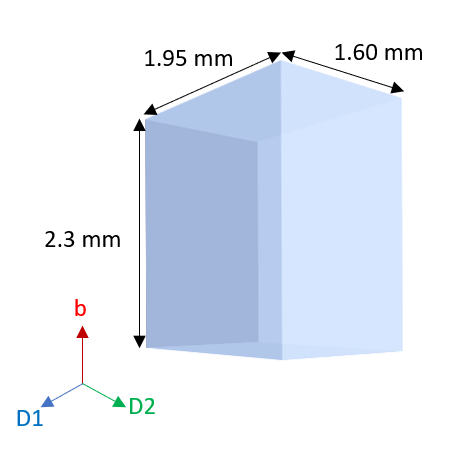
\includegraphics[height=0.4\textwidth,keepaspectratio]{crystaldimesions}
\caption{\label{fig:crystaldimesions} The dimensions of the $^{171}$Yb$^{3+}$:YSO sample used to complete mechanical strain experiments.}
\end{figure}

The magnetisation vector, $\bm{M}$ of excited paramagnetic centres process around $\bm{B_{0}}$ generates a oscillating magnetic field which is detected via the coaxial cable as an AC voltage signal. Typically ESR experiments are completed where the sample are placed into a glass tube holder which is connected to fiberglass rod, where the rod is secured inside the probe such that the sample is in the centre of the resonator. However, in order to investigate the effect of strain on a $^{209}$Bi in isotropically enriched $^{28}$Si in Ref.~\citep{PhysRevLett.120.167701} a costume sample mount was fabricated and connected to the fiberglass rod. The mount was made from a Polyether ether ketone (PEEK) thermoplastic extends into the centre of the cavity. The cylindric hole is drilled into the end of the mount where a fabricated acrylic sample holder secures the isotropic sample. An aluminum base plate which sits on the bottom of cryostat and a second thermoplastic piece extends upwards to meet the mount and also has a milled insert to secure the sample from below. The mount rotates freely and the base remains stationary. 

Due to anisotropy of Yb$^{3+}$ doped in the YSO crystal, the sample mount must be adapted to secure the doped YSO sample which has been cut along the orthogonal dielectric axes. Therefore a separate adapter must be fabricated for each dielectric axis to be orientated perpendicular to $\bm{B_{0}}$ where the crystal dimensions given in Fig.~\ref{fig:crystaldimesions}. Further description of the sample mounting in the cryostat and the sample holder fabrication is presented in the section below.   




\subsection{Fabrication}
\begin{figure}[H]
    \centering
    \begin{subfigure}[b]{0.35\textwidth}
        \centering
 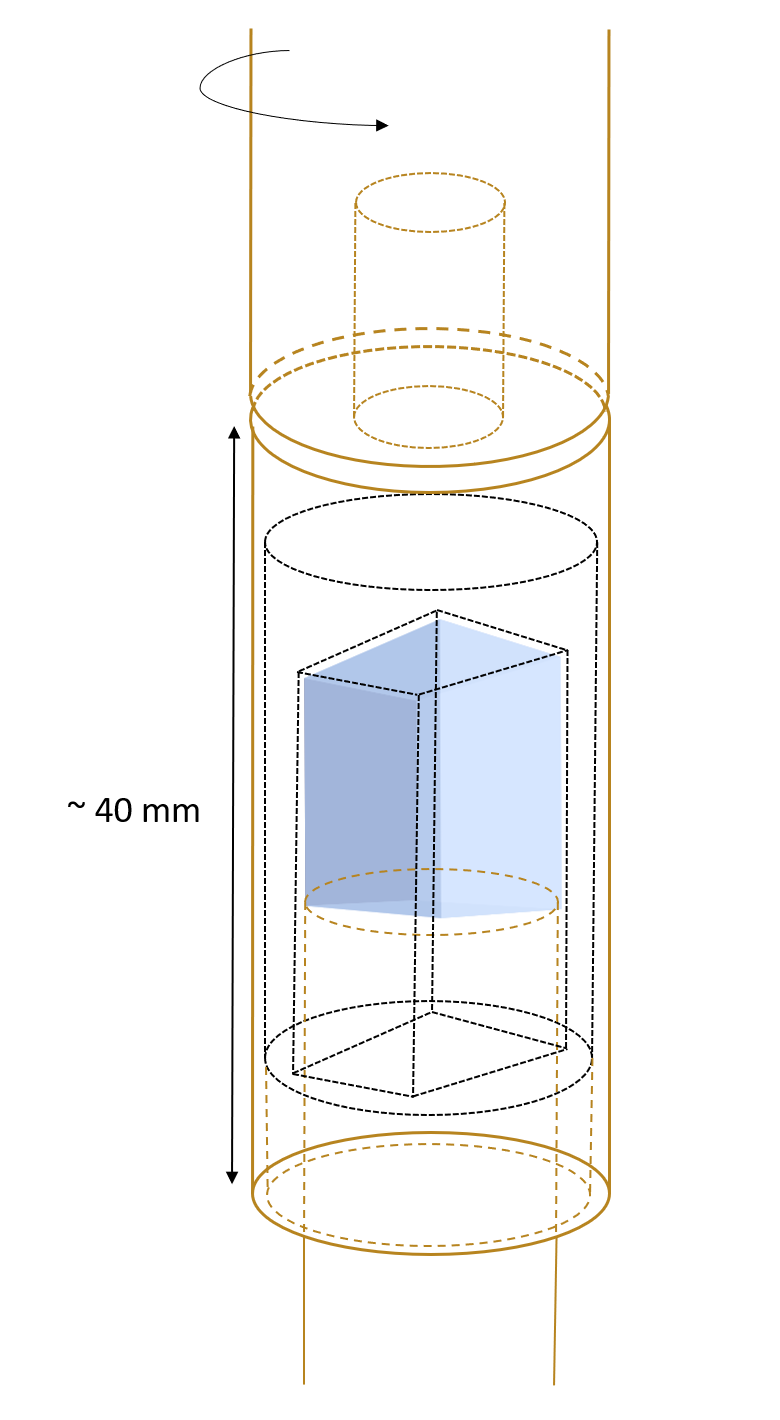
\includegraphics[width=\textwidth]{sampleholder}
       \caption{\label{fig:sampleholder}} 
       \end{subfigure}
%     \hfill
    \begin{subfigure}[b]{0.4\textwidth}
        \centering
        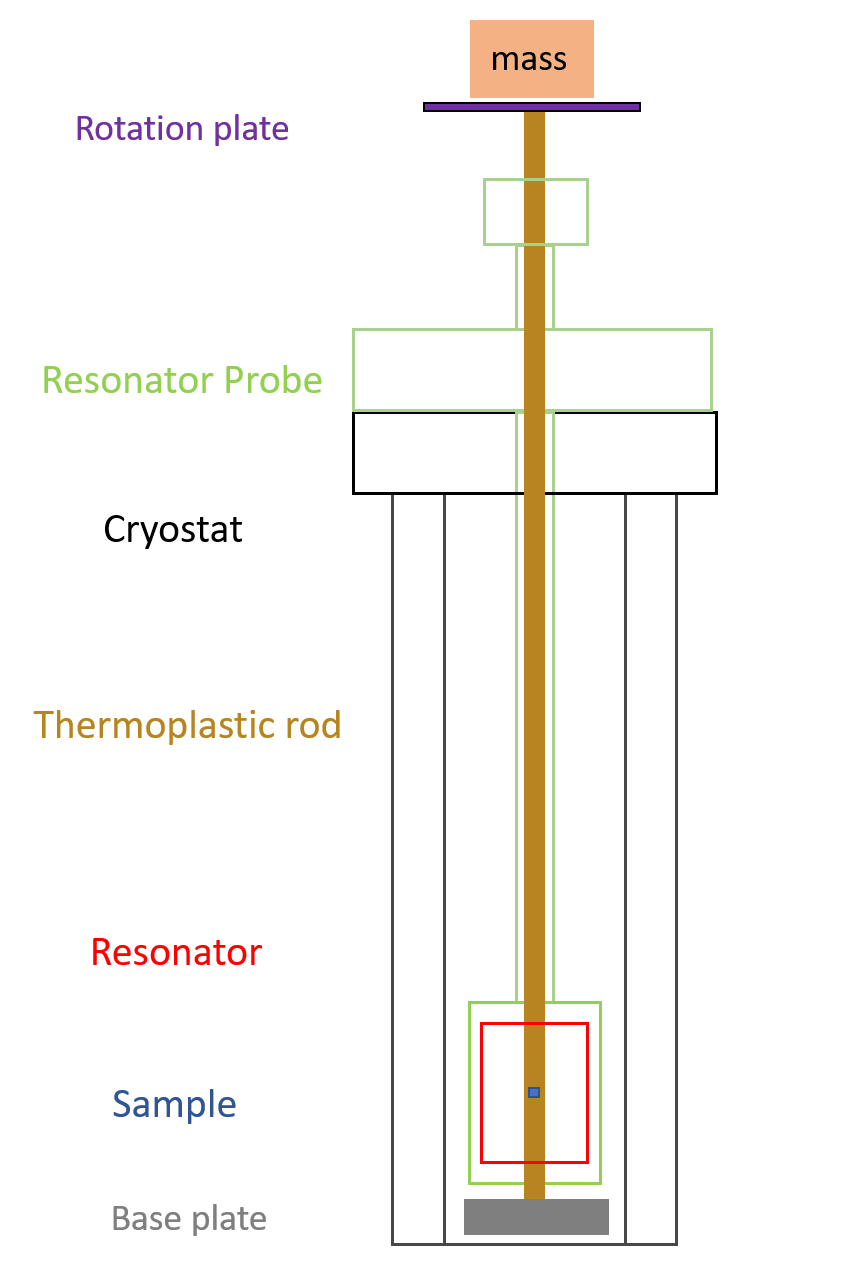
\includegraphics[width=\textwidth]{cryostatschematic}
        \caption{\label{fig:cryostatschematic} }
     \end{subfigure}
    \caption{(a) Illustration of an adapter strain mount for the YSO sample with the b-axis parallel to the rod axis. (b) Schematic of experimental setup showing ESR resonator probe mounted inside liquid Helium flow cryostat. The sample is held in place in the centre of the resonator by fabricated thermoplastic rods.}
\end{figure}

The main thermoplastic rod is connected to the fiberglass rod via a screw. Connection between the adapter and the main rod is obtained by connecting the main thermoplastic piece to the adapter by fabricating a screw and thread. This is done by milling a small recess into to the rod and tapping to create the nut. The adapters are sanded and a die is used to create the bolt. The adapter piece for the sample holder is shown in Fig~\ref{fig:sampleholder} where the cryostat schematic is shown in Fig.~\ref{fig:cryostatschematic}. Similarly a recess is milled in the opposite end of the adapter where, iRoland Modela computer numerical control (CNC) machined, acrylic sample holders are secured within using epoxy resin. To provide further protection against the becoming lost within the cryostat, the new solid thermoplastic piece connected to the base plate is sanded such that it fits within the adapter pieces and thus is secured using cryogenic tape. Therefore, due to do added tape thickness the adapters must be sanded as much as possible to allow free rotation when inside the resonator. Further images of the sample holder and thermoplastic pieces are shown in Appendix~\ref{sec:sampleprobefabrication}.


\subsection{EPR spectrometer}
The EPR spectrometer and MATLAB instrument interface GARII was built by Gary Wolfowicz and further enhanced by Philipp Ross~\citep{mansirthesis}. This device enables AC pulses to be generated which drive transitions between the electron spin states in the sample and additionally to detect the echo signal. The EPR spectrometer schematic is shown in Fig.~\ref{fig:zoidberg}. 

\begin{figure}[h]
\centering
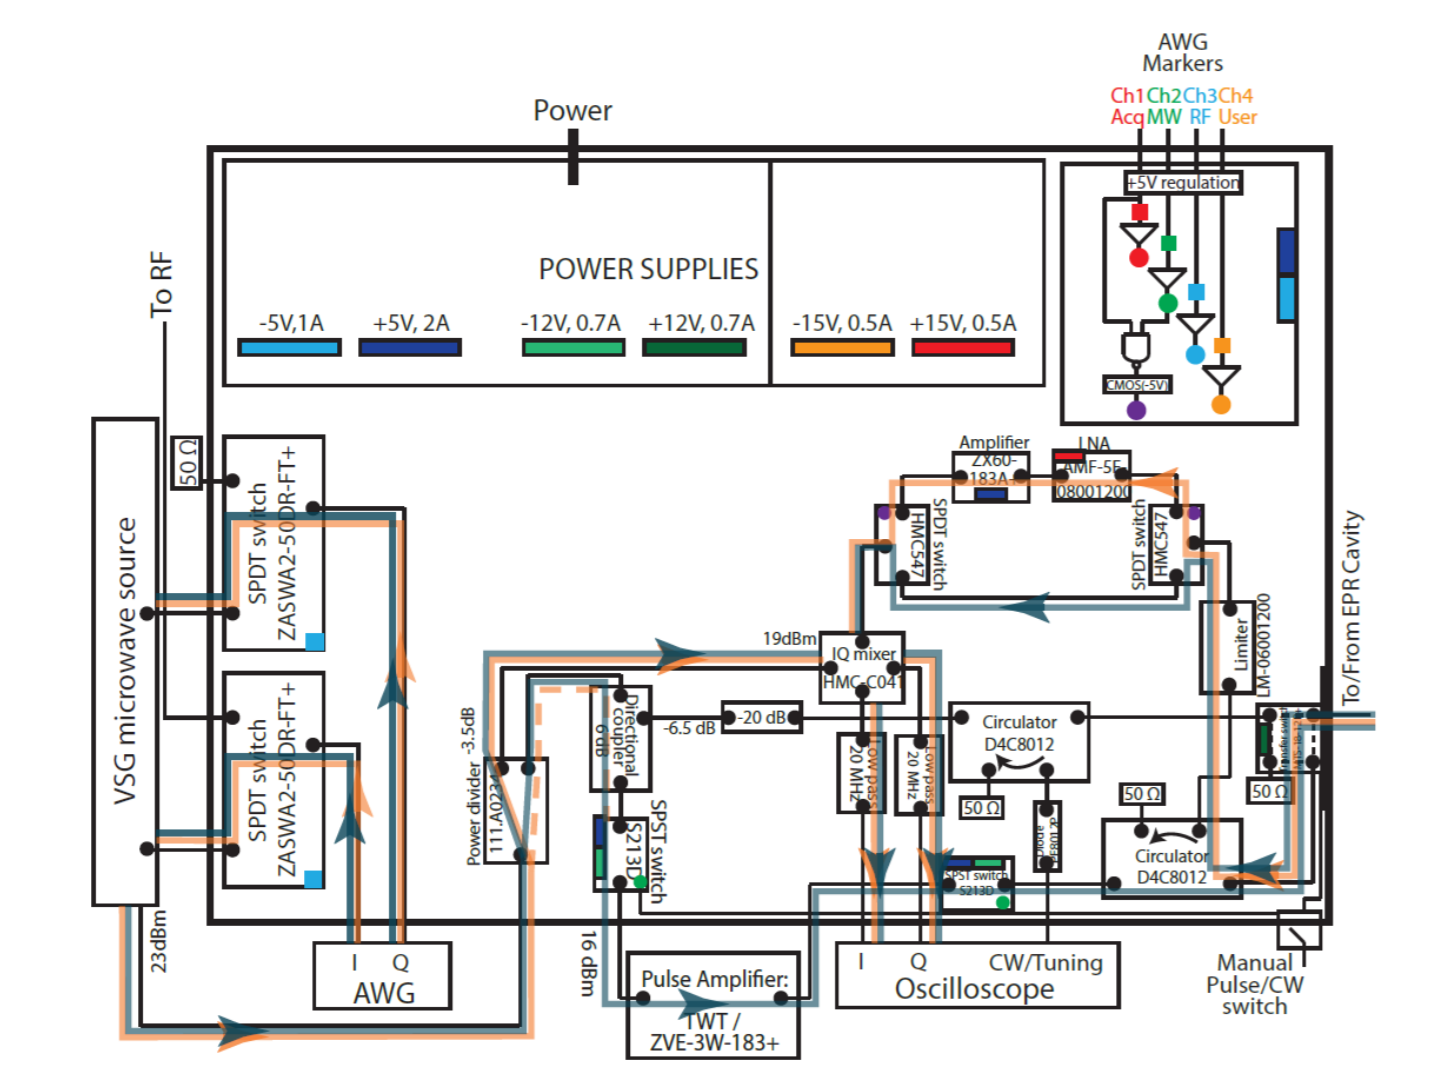
\includegraphics[height=0.5\textwidth,keepaspectratio]{zoidberg}
\caption{\label{fig:zoidberg} EPR spectrometer schematic\citep{mansirthesis}.}
\end{figure}

The $\omega_{MW}$ AC pulse is generated by the vector signal generator (VSG) and modulated using a arbitrary waveform generator. The signal amplitude is controlled by using a TWT amplifier and attenuator. The high power pulse is then sent via the circulator to the coaxial antenna. During the acquisition time window the protection switch is set such that the weak response echo signal is transmitted to the low-noise amplifier (LNA). Therefore during experimental set-up the attenuated must be reduced in integer dB steps whilst and MW pulses are inspected to ensure there is no pulse ringing in the acquisition window as this could damage the sensitive electronic components. The amplified detection signal is then sent to a quadrature mixer with the reference VSG signal where demodulation of the in-phase (I) and out-of-phase (Q) components are displayed by the oscilloscope~\citep{goldfarb2018epr}. 



\section{\label{sec:simulation}Simulation}
The MATLAB toolbox EasySpin was used to simulate the electron paramagnetic spectra used to guide the experimental measurements for this project. Information about the crystal symmetry, the rare-earth ion electron and nuclear spin quantum number the tensors determined by Welinski~\citep{PhysRevB.94.155116}, presented in Section.~\ref{sec:YSOdopedYbions}, was inputted. This allows properties of $^{171}$Yb$^{3+}$:YSO to be probe computationally through the use of spin Hamiltonian solvers. The energy level transitions can be obtained depending on the orientation of the static magnetic field, where the case for $\bm{B_{0}}$ along the D1-axis is shown in Fig~\ref{fig:energylevsim} for each crystal site. 


\begin{figure}[H]
    \centering
    \begin{subfigure}[b]{0.4\textwidth}
        \centering
        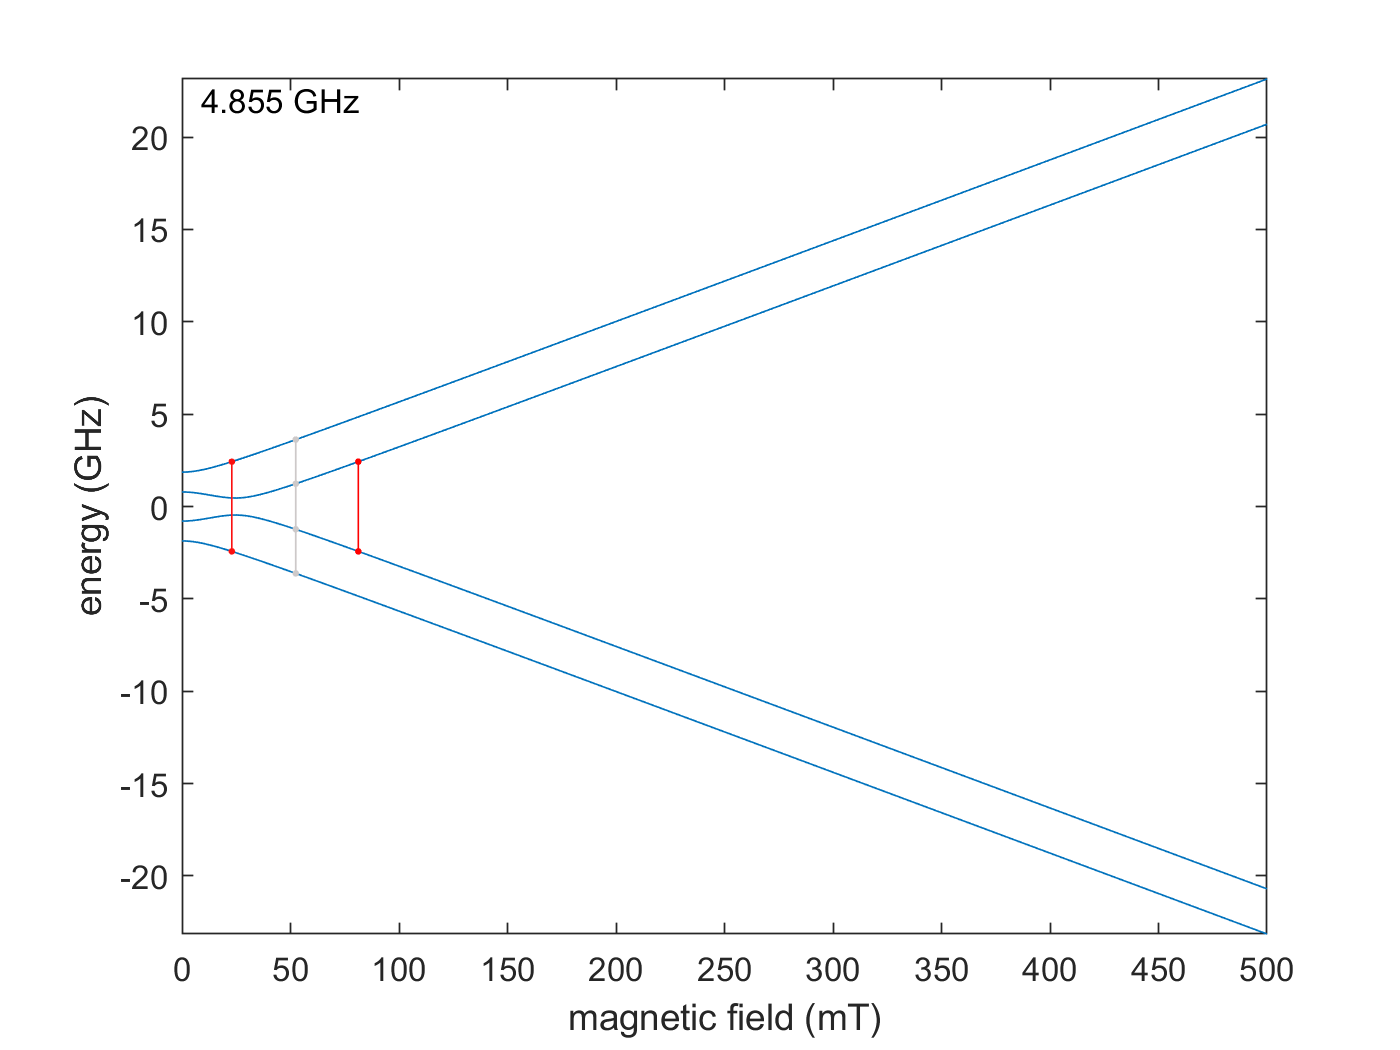
\includegraphics[width=\textwidth]{site1energylevels}
        \caption{}
    \end{subfigure}
%     \hfill
    \begin{subfigure}[b]{0.4\textwidth}
        \centering
        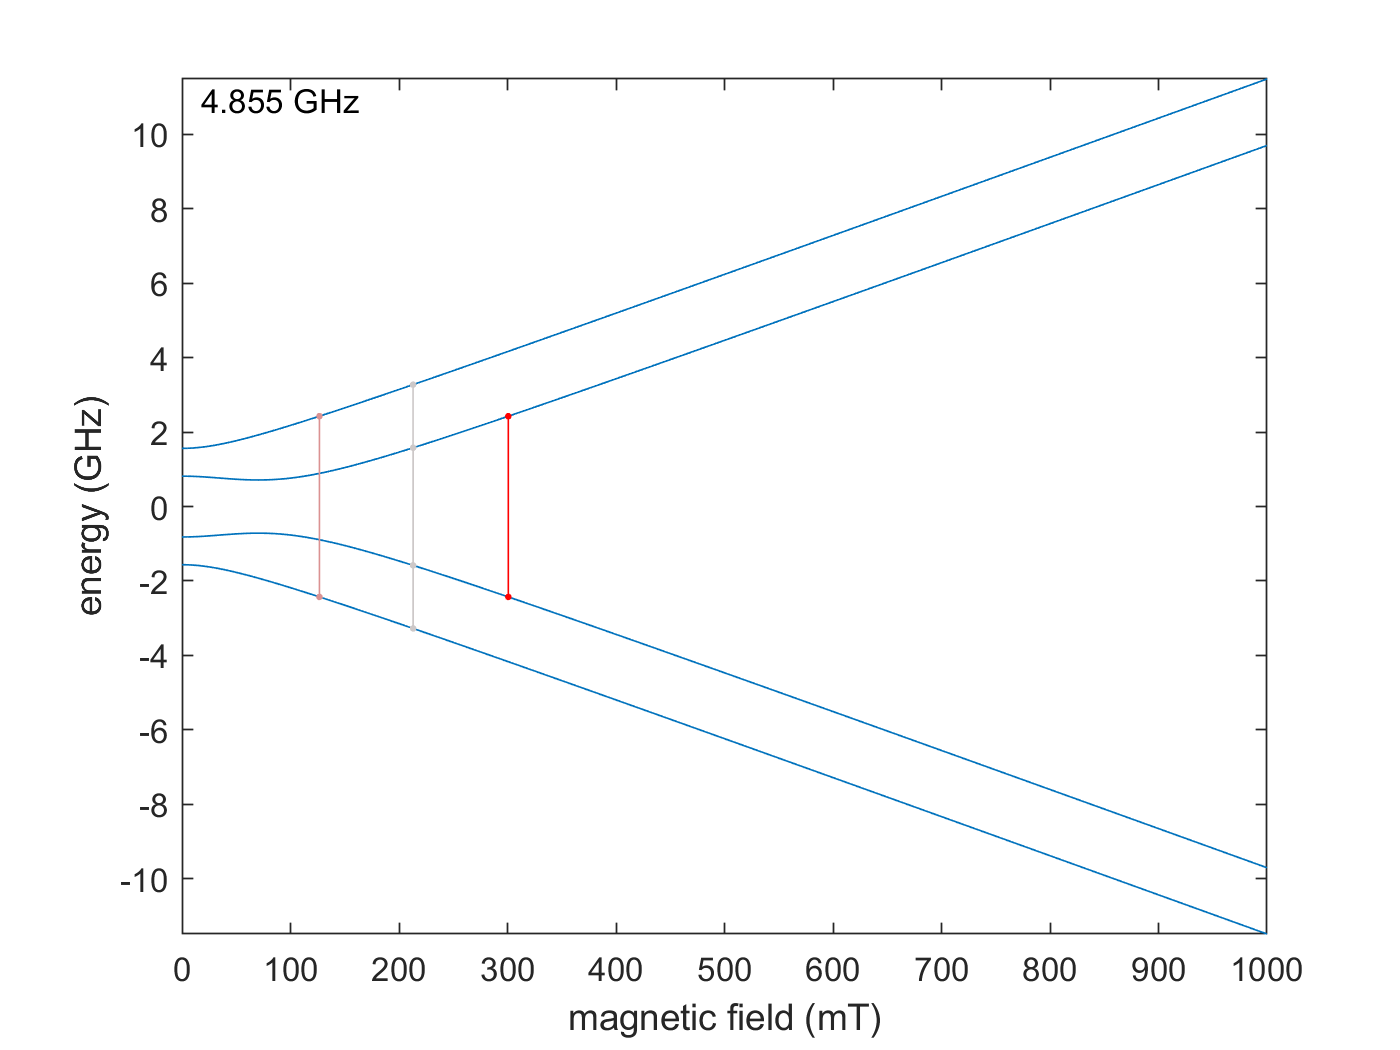
\includegraphics[width=\textwidth]{site2energylevels}
   \caption{}
   \end{subfigure}
   \caption{$^{171}$Yb:YSO energy spectra as a function of the strength of $B_{0}$ along the D1 axis for (a) site I and (b) site II. Transition between allowed (red) and disallowed (grey) eigenstates are shown for a resonator frequency of 9.63 GHz.}
   \label{fig:energylevsim}
\end{figure}


\begin{figure}[H]
    \centering
    \begin{subfigure}[b]{0.46\textwidth}
        \centering
        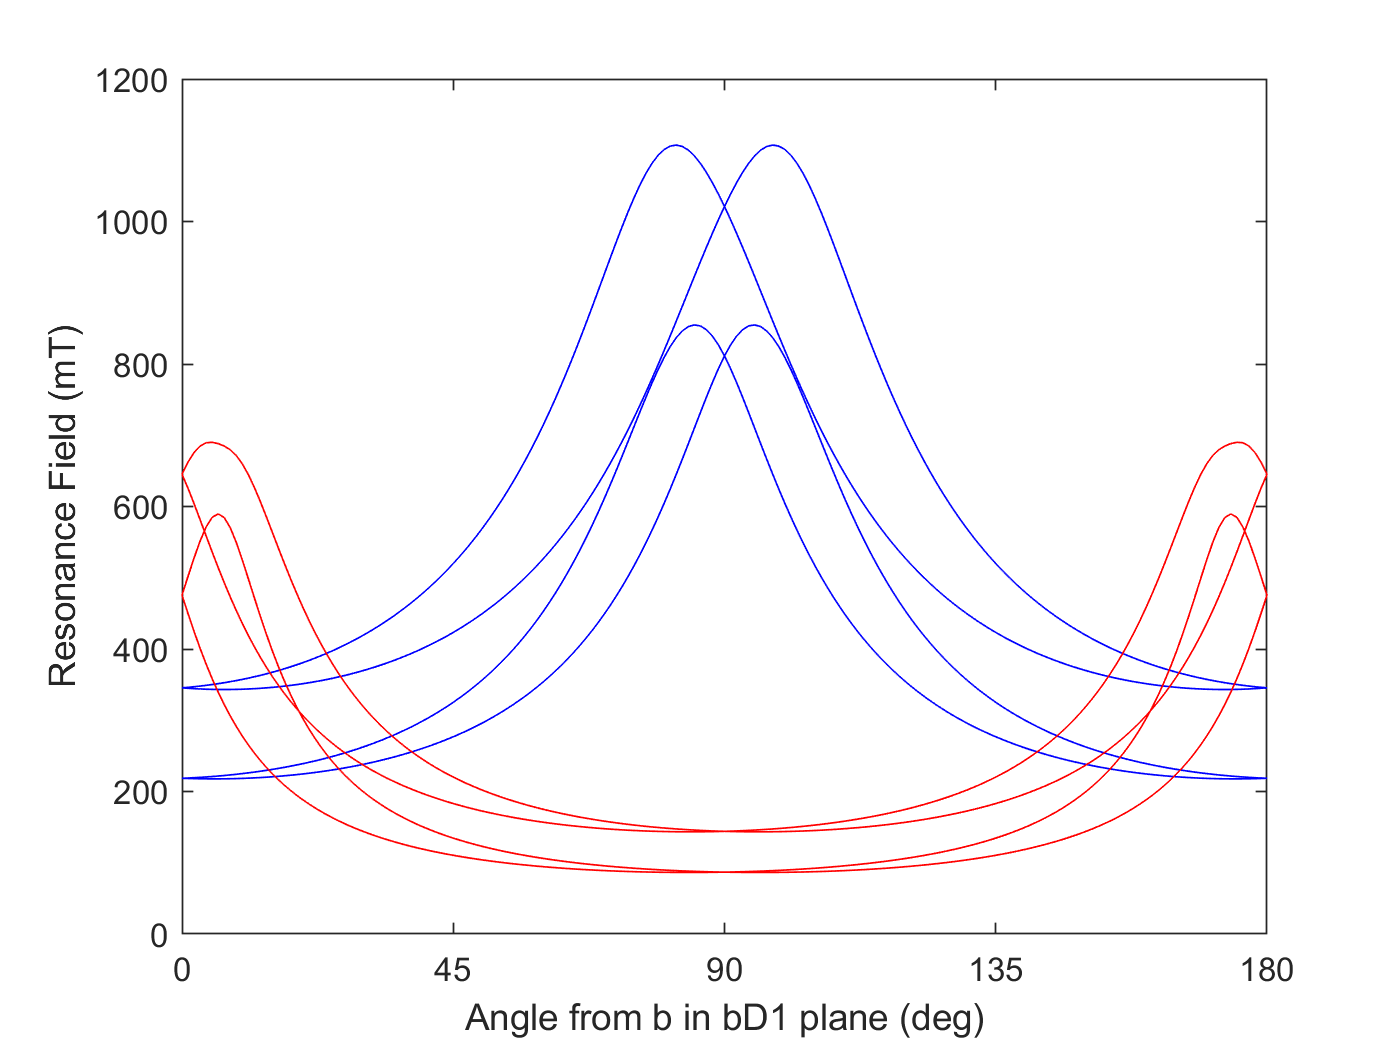
\includegraphics[width=\textwidth]{frombinbD1plane}
        \caption{\label{fig:simmagresori1}}
    \end{subfigure}
%     \hfill
    \begin{subfigure}[b]{0.3\textwidth}
        \centering
        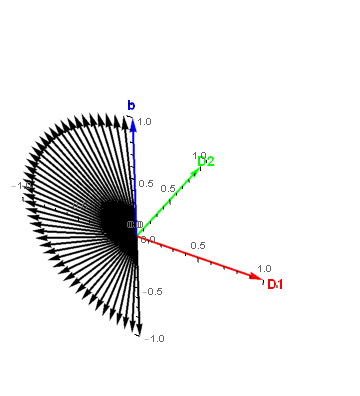
\includegraphics[width=\textwidth]{BperD2}
   \caption{}
   \end{subfigure}
       \begin{subfigure}[b]{0.46\textwidth}
        \centering
        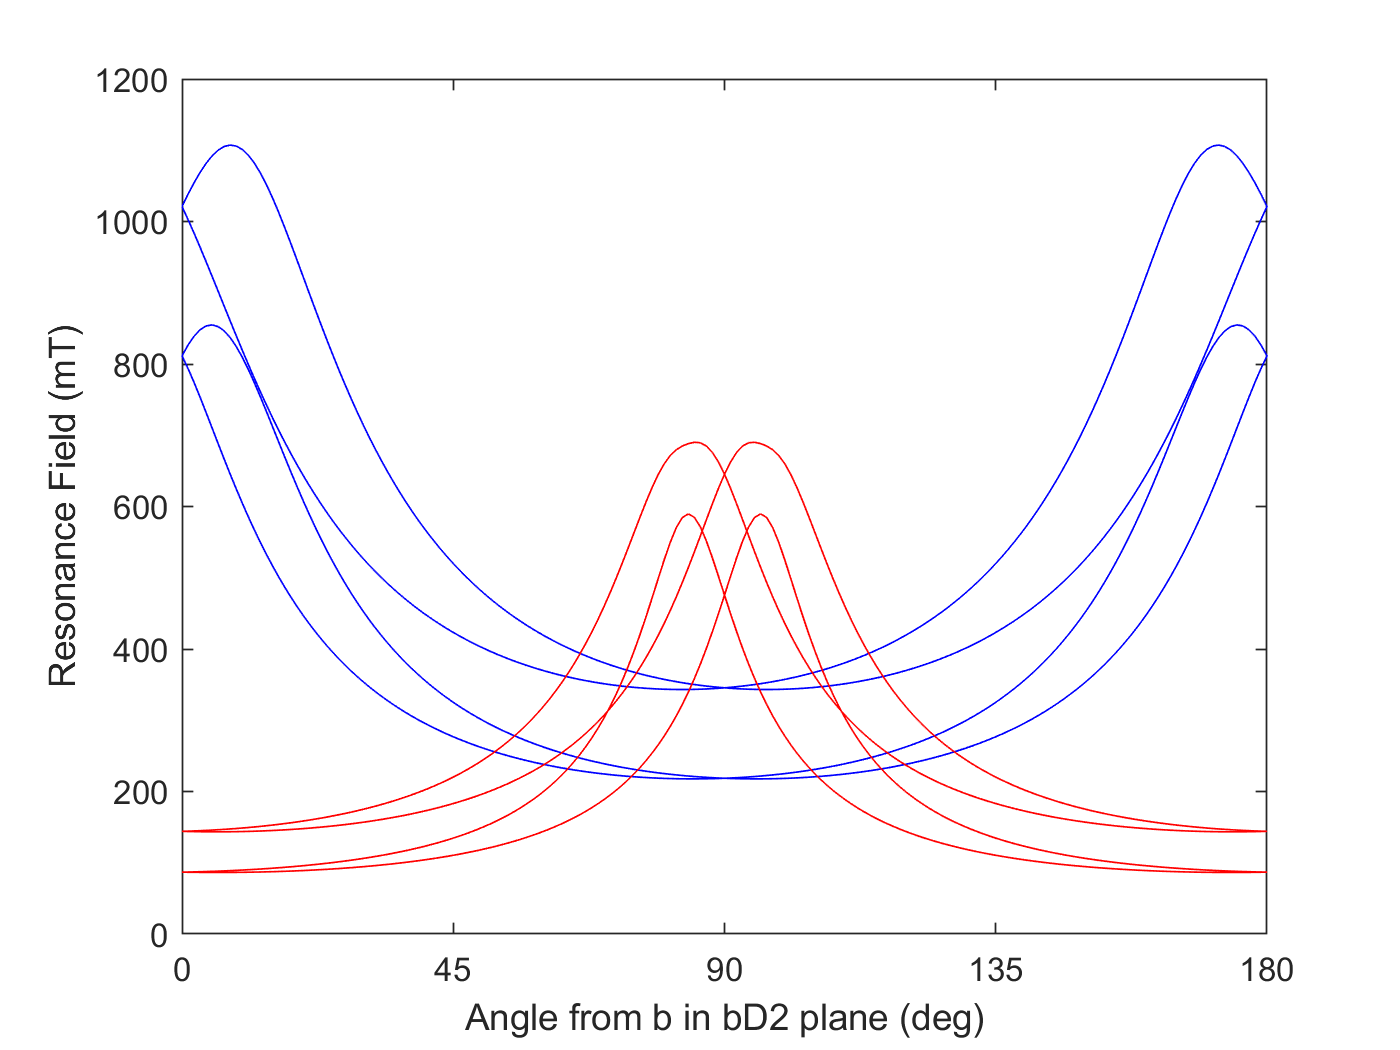
\includegraphics[width=\textwidth]{frombinbD2plane}
   \caption{\label{fig:simmagresori2}}
   \end{subfigure}
       \begin{subfigure}[b]{0.3\textwidth}
        \centering
        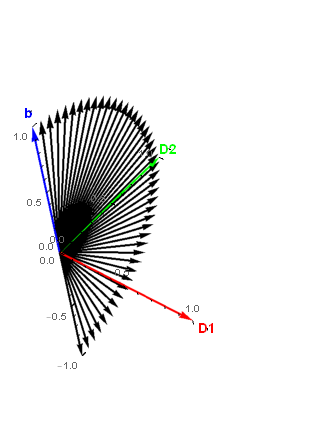
\includegraphics[width=\textwidth]{BperpD1}
   \caption{}
   \end{subfigure}
       \begin{subfigure}[b]{0.46\textwidth}
        \centering
        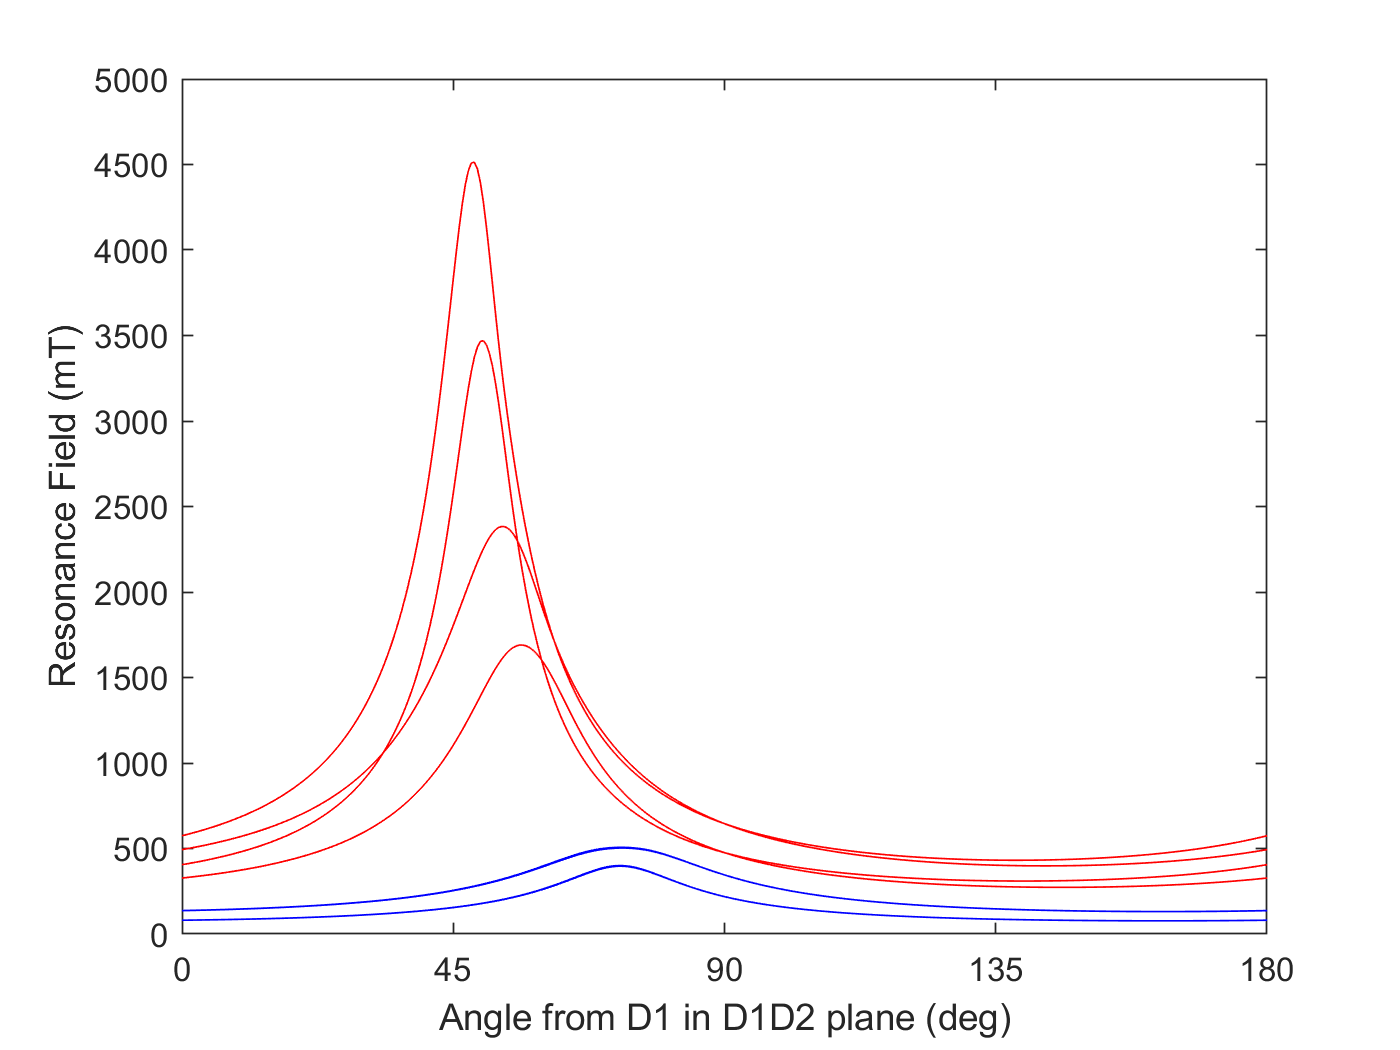
\includegraphics[width=\textwidth]{fromD1inD1D2plane}
   \caption{\label{fig:simmagresori3}}
   \end{subfigure}
       \begin{subfigure}[b]{0.3\textwidth}
        \centering
        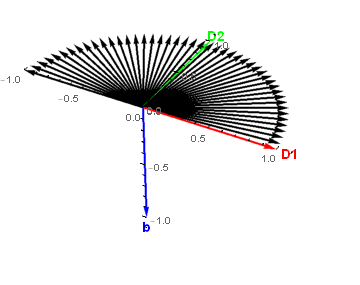
\includegraphics[width=\textwidth]{Bperb}
   \caption{}
   \end{subfigure}
   \caption{The resonant magnetic field for $^{171}$Yb:YSO as a function of orientation is shown in (a),(c) and (e) where magnetic field relative to the dielectric axes is displayed in (b),(d) and (f), respectively. Site I is shown in blue and site II is shown in red.}
   \label{fig:simmagresori}
\end{figure}

To investigate the resonant magnetic field as a function of the orientation of the sample I firstly, as shown in Appendix~\ref{sec:easyspinsim}, reproduced the results in Ref.~\citep{mairflaig} for $145$Nd$^{3+}$ doped YSO. Thereafter, the magnetic field resonance vs. orientation is computed which is good agreement with the experimentally measured values in Ref.~\citep{PhysRevB.94.155116}. The sub-site magnetic field degeneracies are lifted as the orientation is varied as shown in Fig.~\ref{fig:simmagresori}. To obtain magnetic field splitting for Fig~\ref{fig:simmagresori3} a small $R_{y}$ rotation of the initial magnetic field vector is included since there is a small error ($\approx$2$^{\circ}$) is associated with cutting the sample along the dielectric axes~\citep{PhysRevB.94.155116}.    


\begin{figure}[H]
    \centering
    \begin{subfigure}[b]{0.45\textwidth}
        \centering
        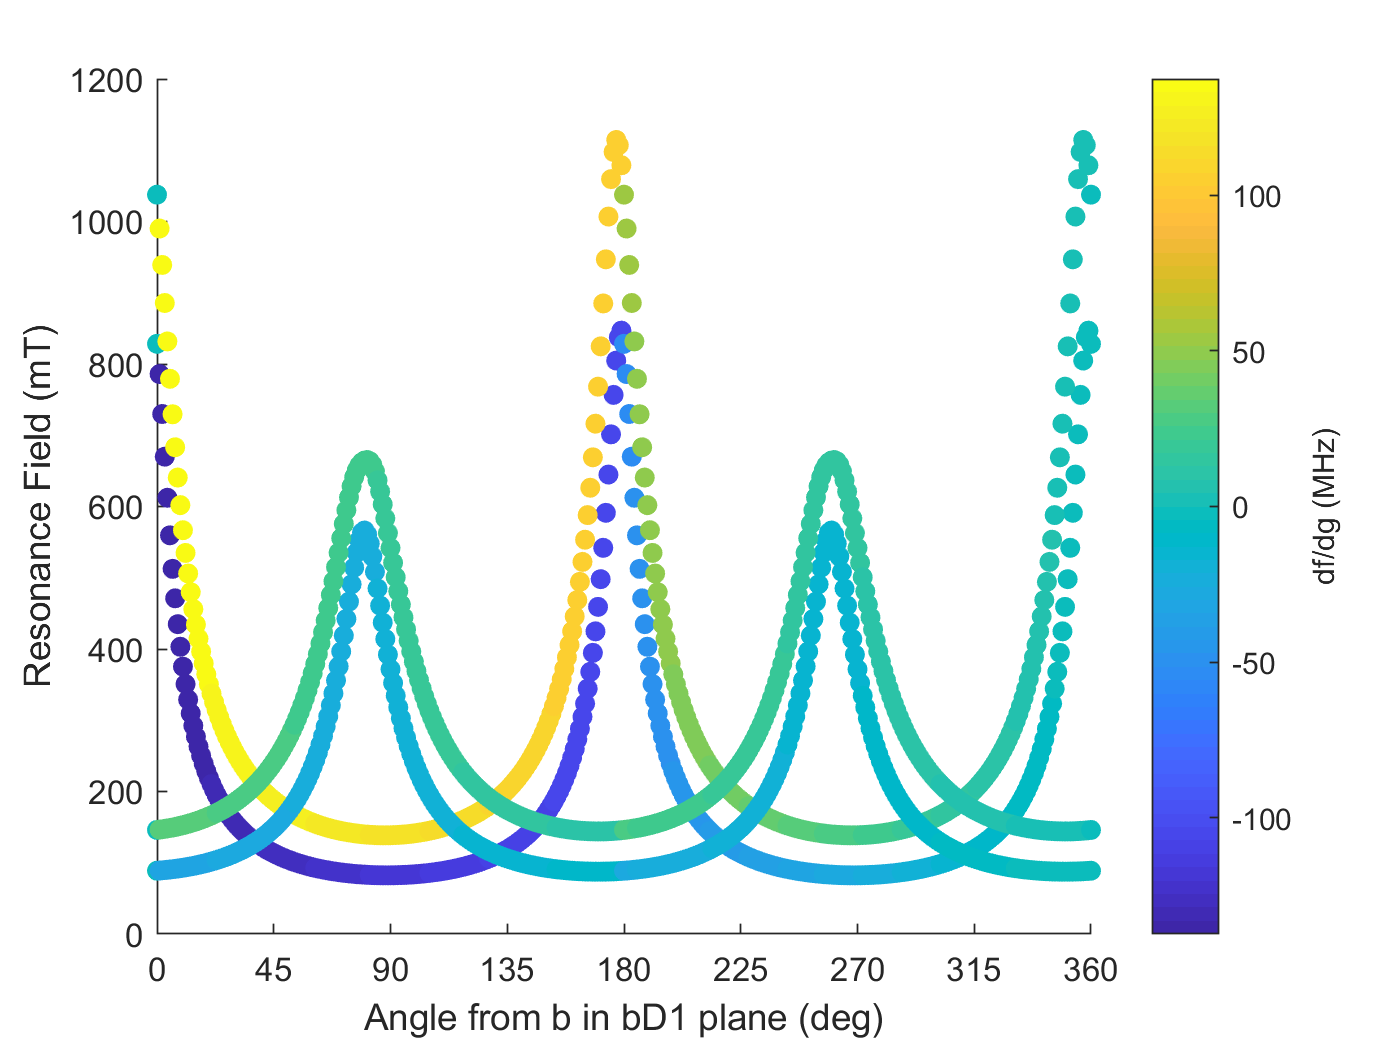
\includegraphics[width=\textwidth]{pertanglebinbD1plane}
        \caption{\label{fig:simmagresori1}}
    \end{subfigure}
%     \hfill
    \begin{subfigure}[b]{0.45\textwidth}
        \centering
        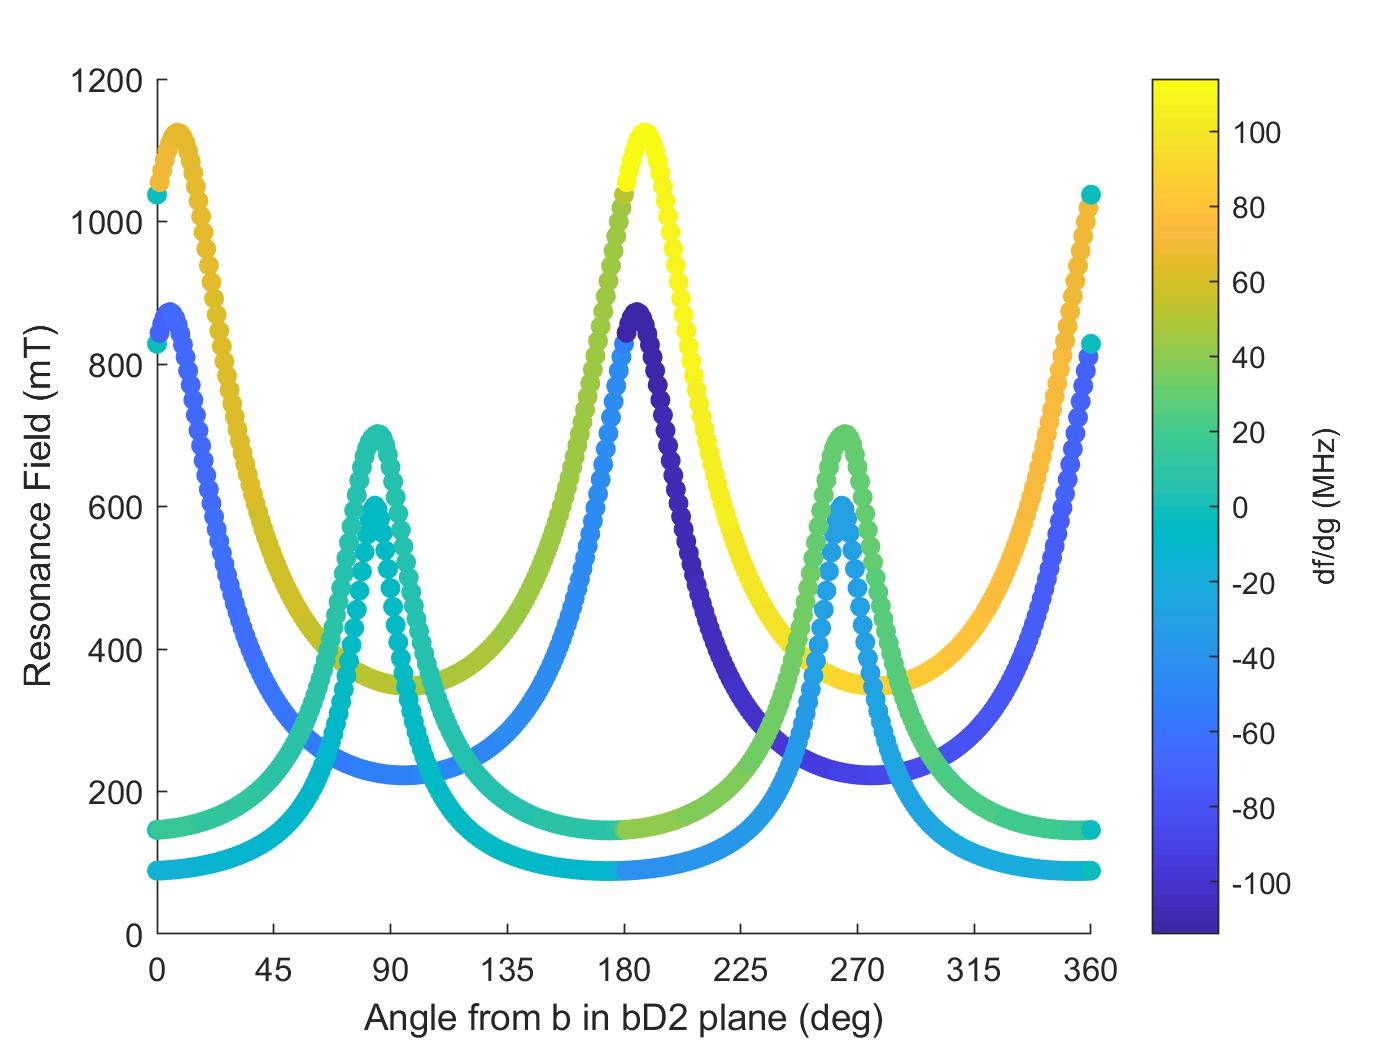
\includegraphics[width=\textwidth]{pertanglebinbD2plane}
   \caption{}
   \end{subfigure}
       \begin{subfigure}[b]{0.45\textwidth}
        \centering
        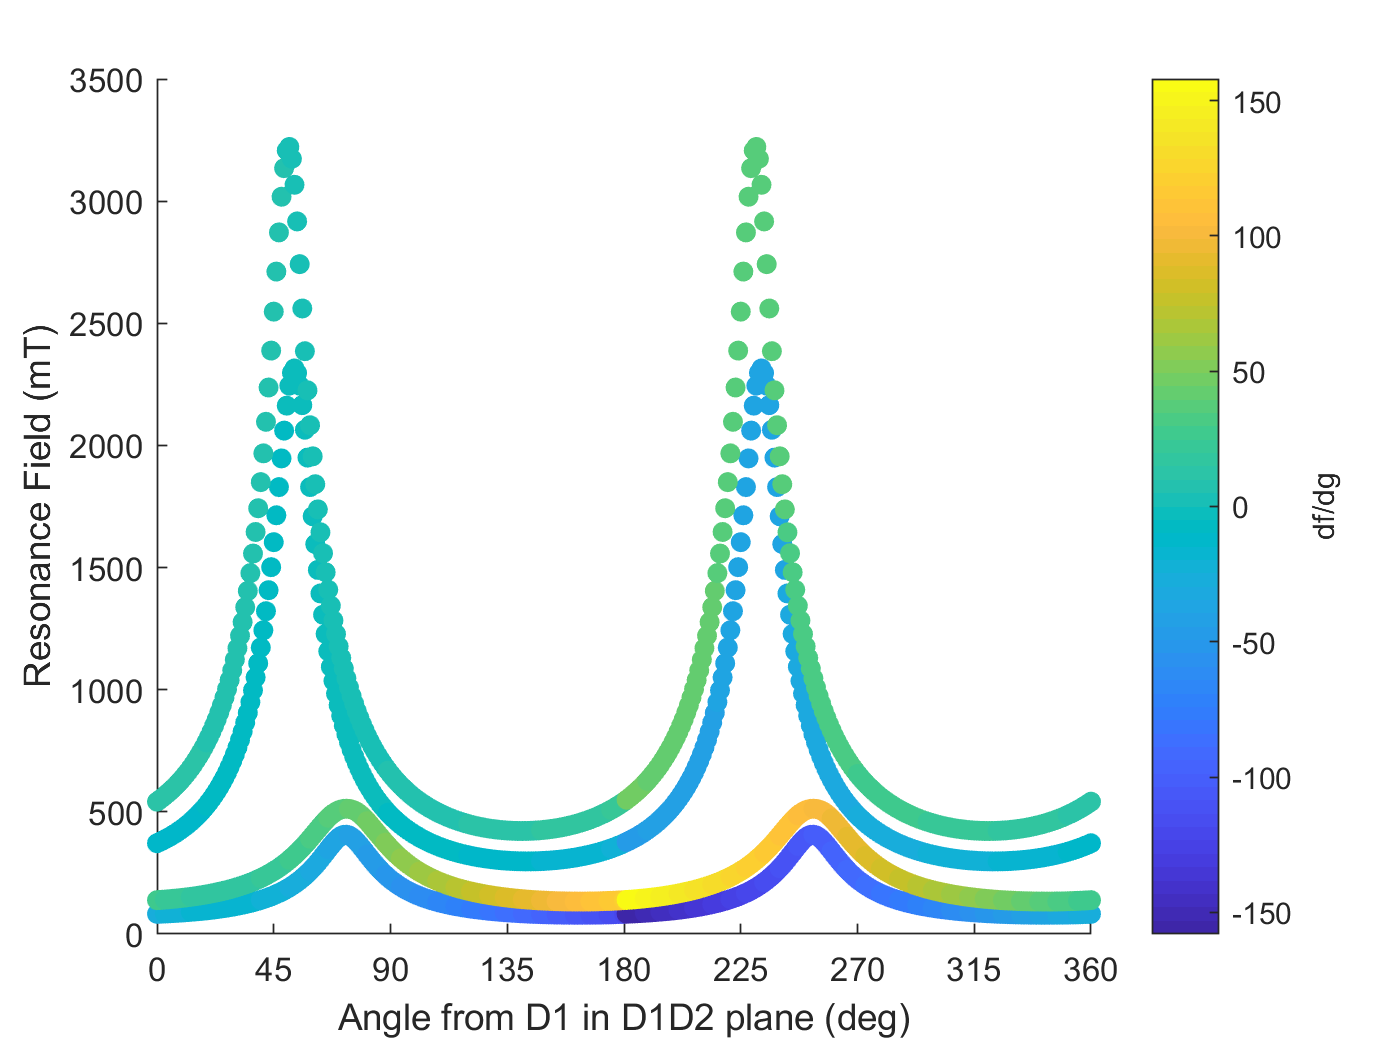
\includegraphics[width=\textwidth]{pertangleD1inD1D2plane}
   \caption{\label{fig:simmagresori2}}
   \end{subfigure}
   \caption{Angular variations of the EPR transitions for $^{171}$Yb:YSO where the colour bar represents $\Delta f/\Delta g$ for isotropic $\Delta g = 0.05$. Where $\bm{B_{0}}$ is perpendicular to the (a) D2-axis, (b) D1-axis and the (c) b-axis.}
   \label{fig:dfdg}
\end{figure}


\begin{figure}[H]
    \centering
    \begin{subfigure}[b]{0.45\textwidth}
        \centering
        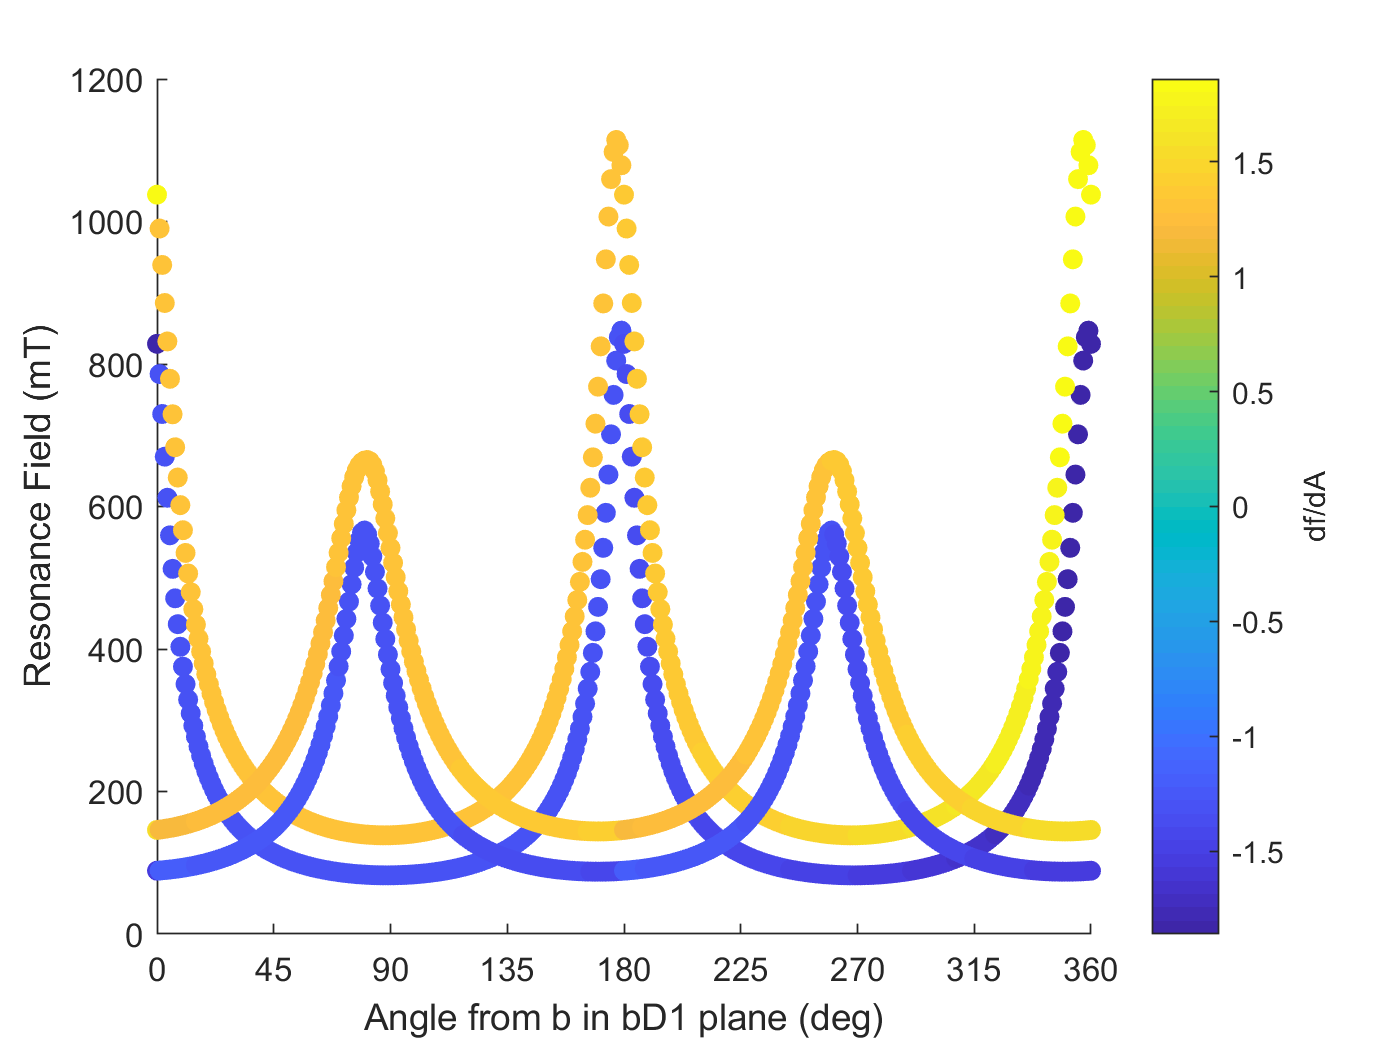
\includegraphics[width=\textwidth]{pertAanglebinbD1plane}
        \caption{\label{fig:simmagresori1}}
    \end{subfigure}
%     \hfill
    \begin{subfigure}[b]{0.45\textwidth}
        \centering
        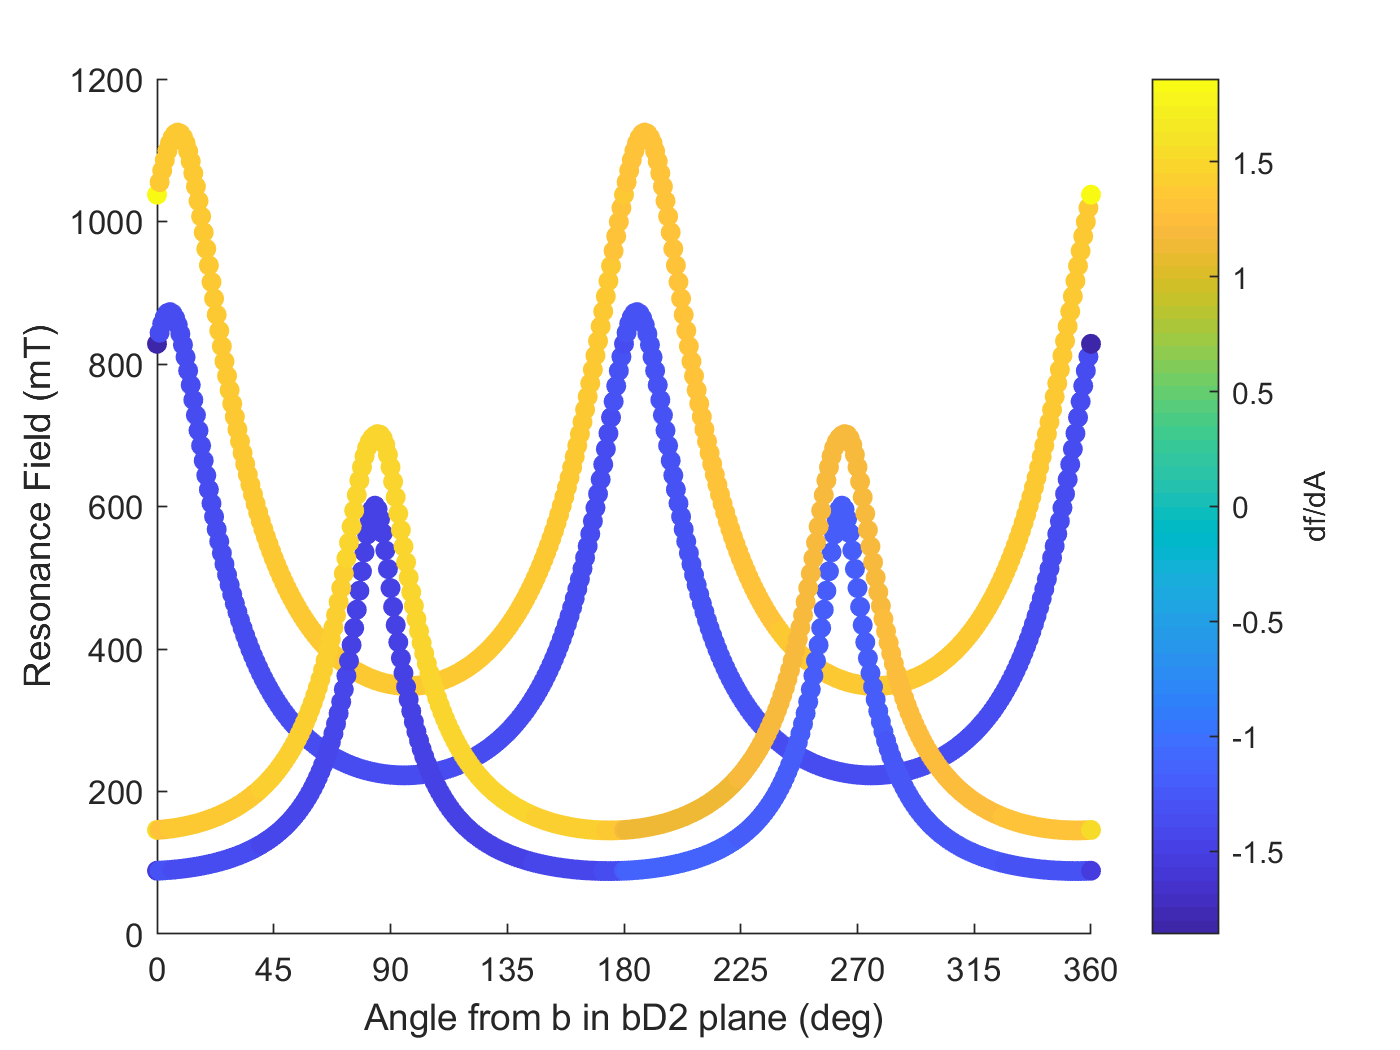
\includegraphics[width=\textwidth]{pertAanglebinbD2plane}
   \caption{}
   \end{subfigure}
       \begin{subfigure}[b]{0.45\textwidth}
        \centering
        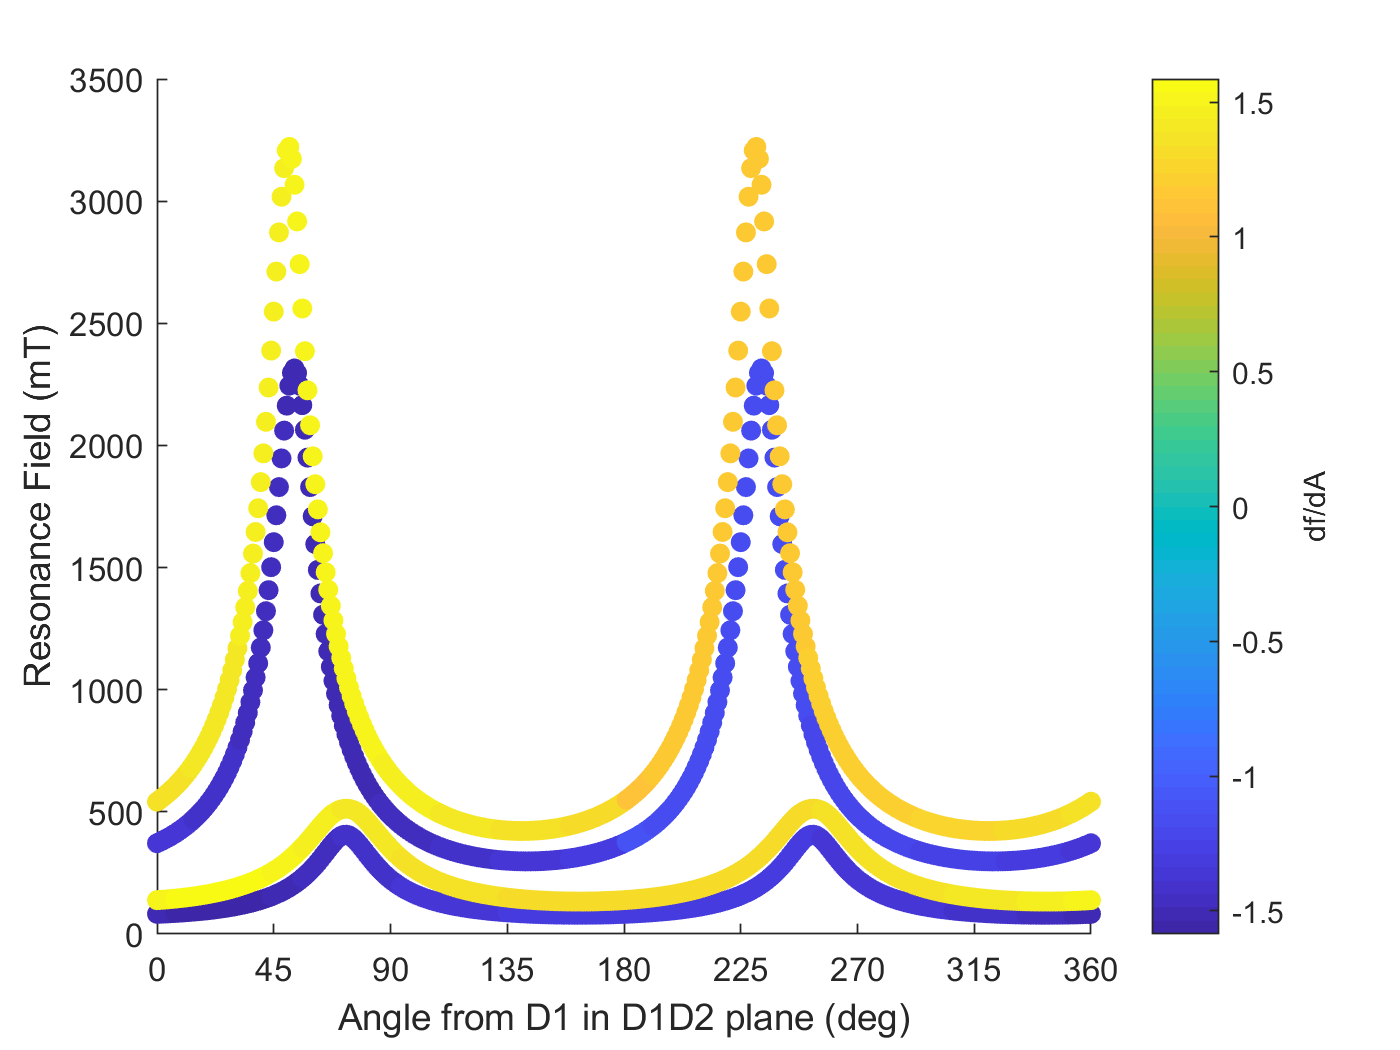
\includegraphics[width=\textwidth]{pertAangleD1inD1D2plane}
   \caption{\label{fig:simmagresori2}}
   \end{subfigure}
   \caption{Angular variations of the EPR transitions for $^{171}$Yb:YSO where the colour bar represents $\Delta f/\Delta A$ for isotropic $\Delta A = 50$ MHz. Where $\bm{B_{0}}$ is perpendicular to the (a) D2-axis, (b) D1-axis and the (c) b-axis.}
   \label{fig:dfdA}
\end{figure}

Furthermore, the calculated change in resonance frequency, $\Delta f$ in response to a small perturbation of either $\bm{g}$ and $\bm{A}$ was explored. The case of an isotropic perturbation of $\Delta g = 0.05$ and $\Delta A = 50$ MHz for each site is shown in Fig.~\ref{fig:dfdg} and Fig.~\ref{fig:dfdA}, respectively. This case simulates the expected effect of isotropic strain. Additionally cases of uniaxial perturbation of $\bm{g}$ and $\bm{A}$ were simulated. However, in reality due the number of nonzero stiffness matrix terms of YSO and unknown $\bm{\mathcal{G}}$ and $\bm{\mathcal{A}}$ tensors, the response of $\bm{g}$ and $\bm{A}$ to uniaxial strain in YSO remains undisclosed. Therefore these simulations provide a preliminary guidance of which crystal orientation to probe.





%This research aims to provide a companion to the investigation of the effect of mechanical strain applied to a group V doped $^28$Si presented in Ref.~\citep{doi:10.1063/1.4919761}. 
